\section{Introduction}

        \subsection{Catastrophic Forgetting in Neural Networks}

        \begin{frame}
            \frametitle{Neural Network}
            \framesubtitle{Training}

            \begin{figure}[H]
                \centering
                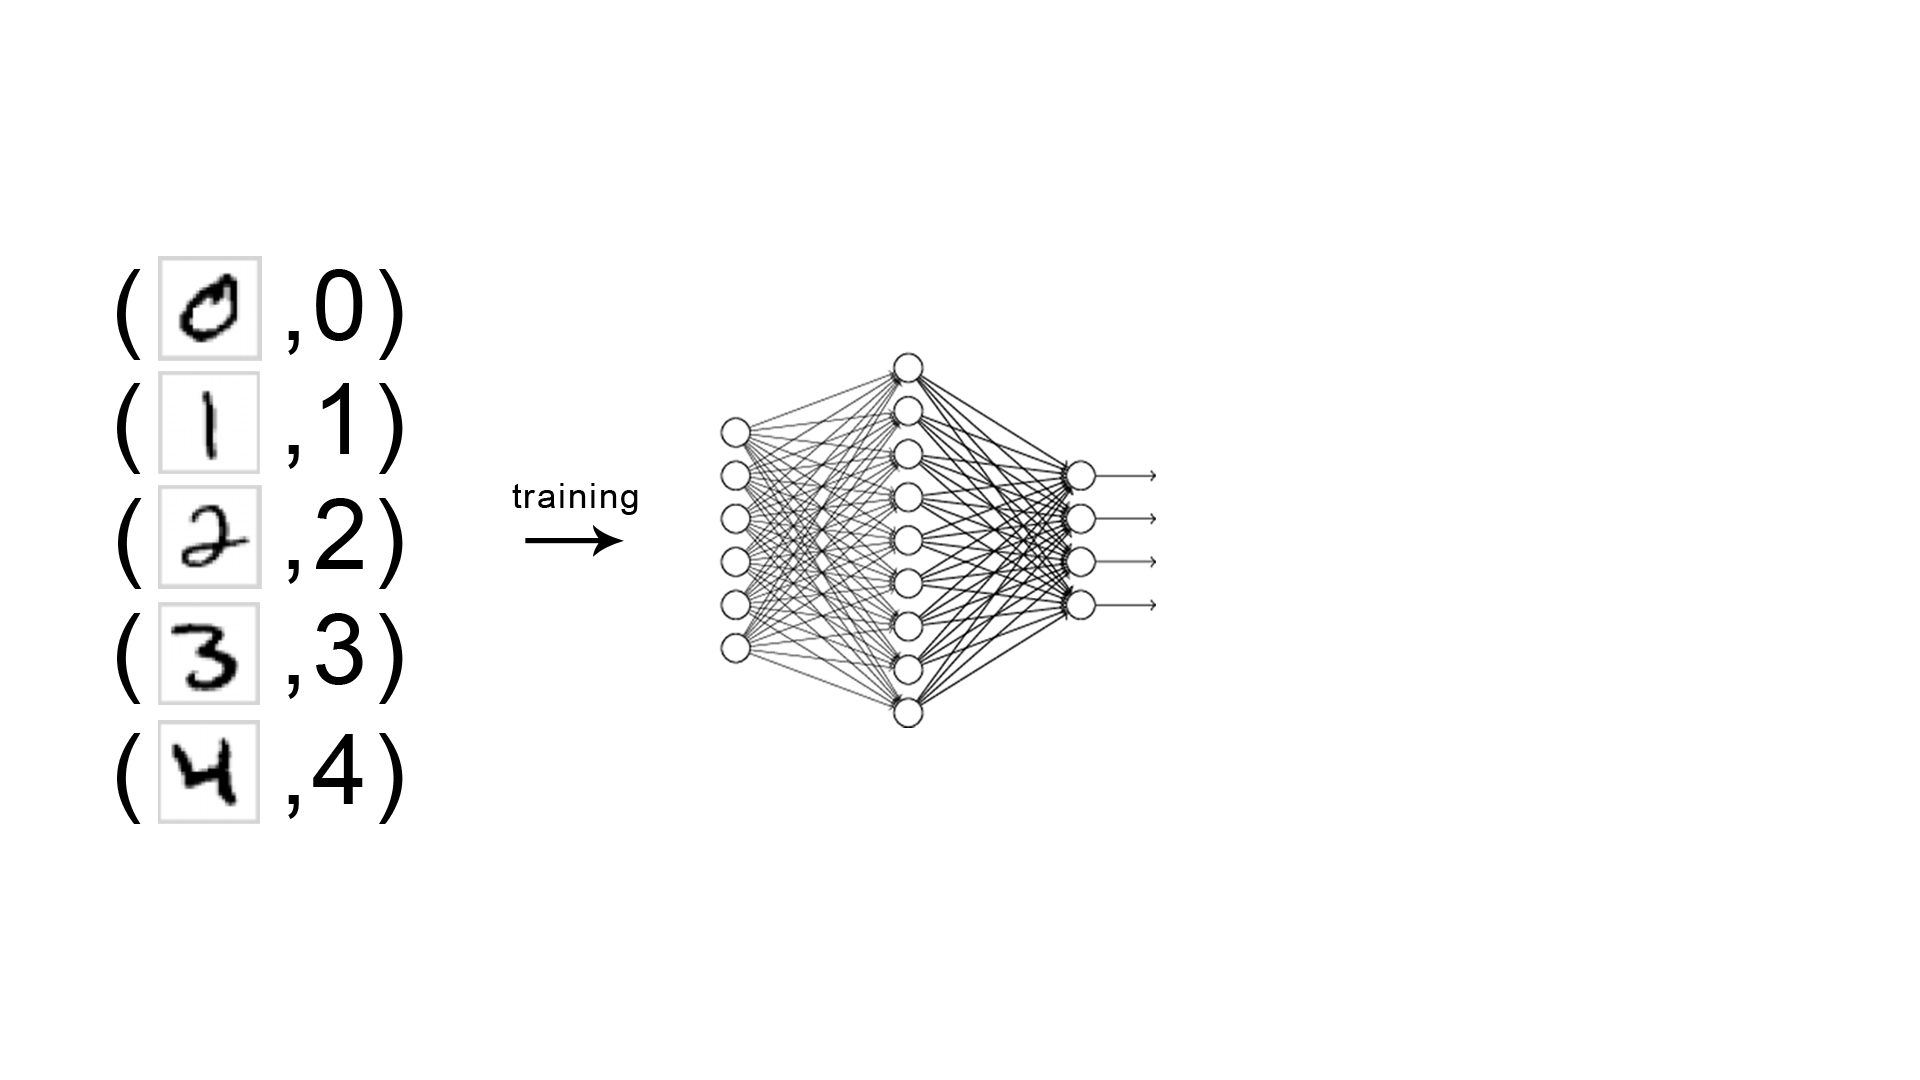
\includegraphics[width=\textwidth]{training_preview}
            \end{figure}
            \footnotetext{\cite{dnn_neuron_basic_overview}}
        \end{frame}
        \begin{frame}
            \frametitle{Neural Network}
            \framesubtitle{Training}

            \begin{figure}[H]
                \centering
                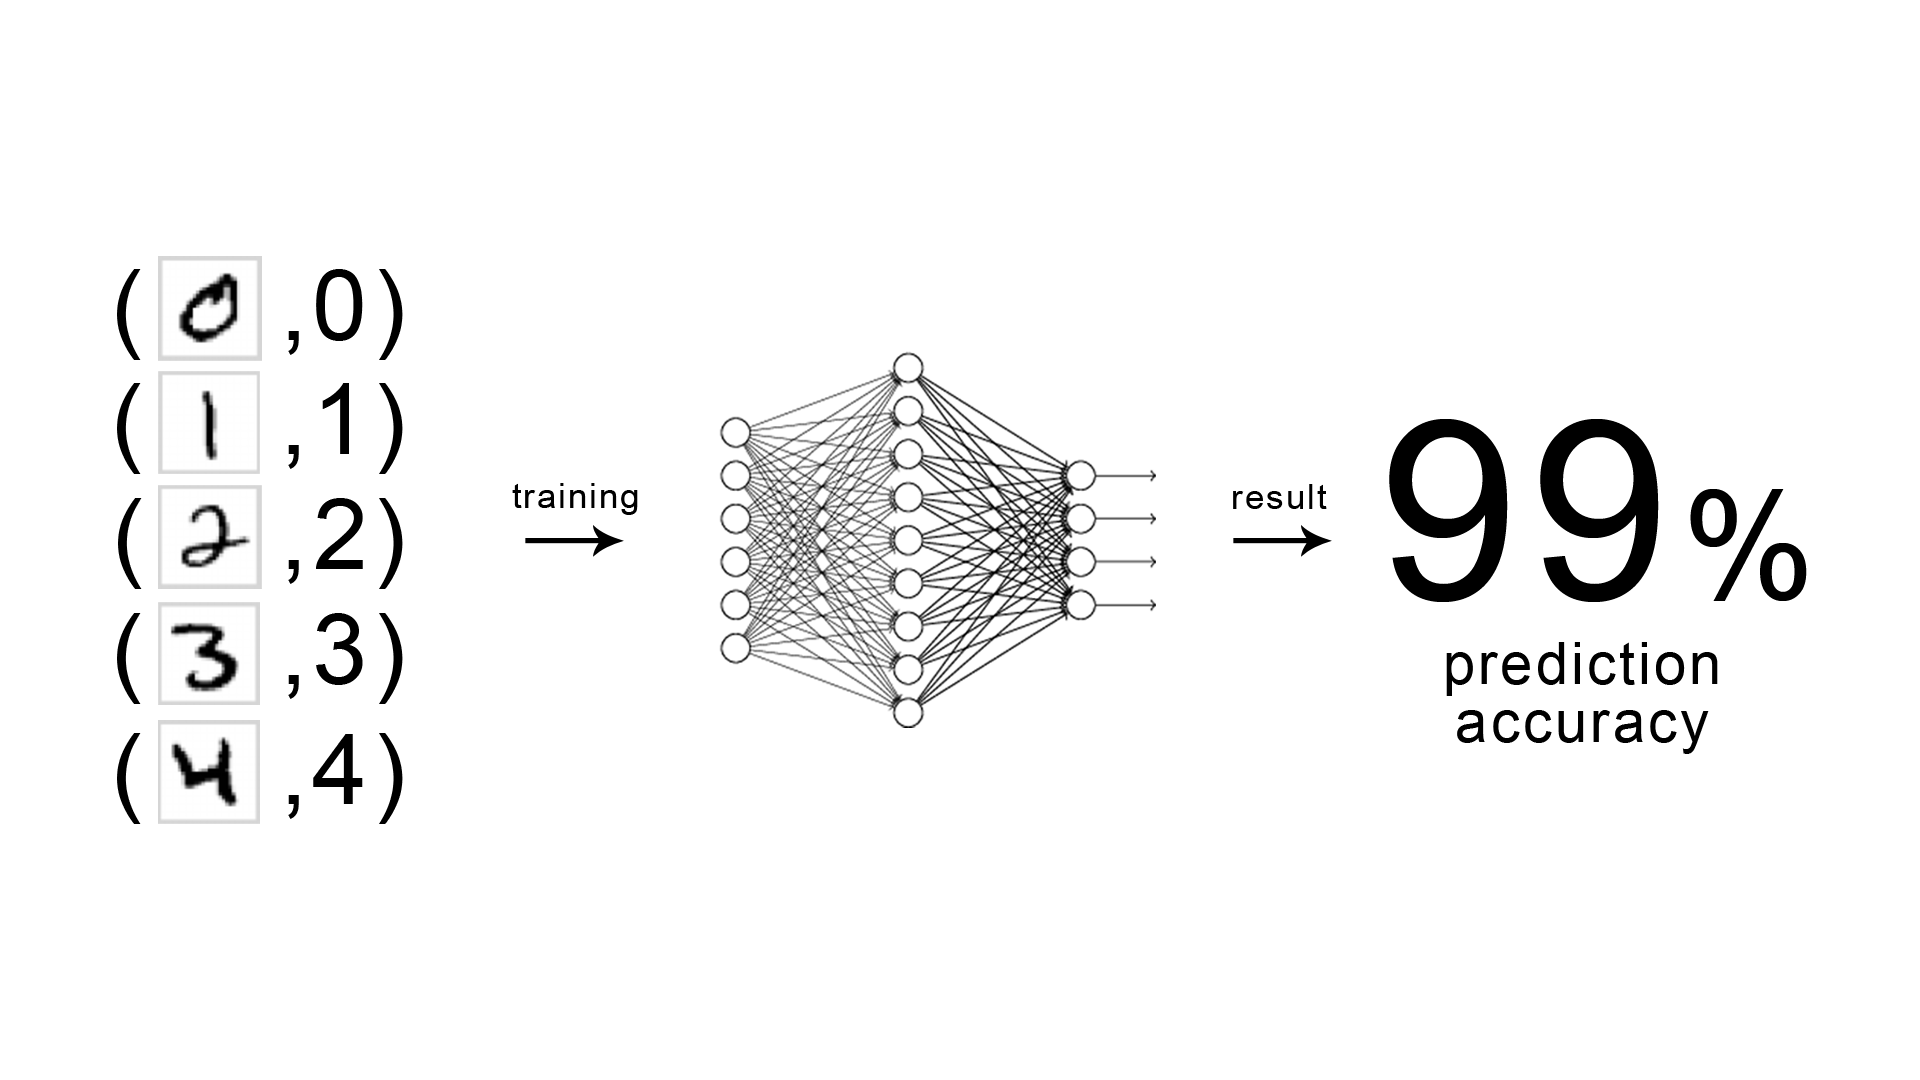
\includegraphics[width=\textwidth]{training_result}
            \end{figure}
        \end{frame}

        \begin{frame}
            \frametitle{Neural Network}
            \framesubtitle{Retraining}

            \begin{figure}[H]
                \centering
                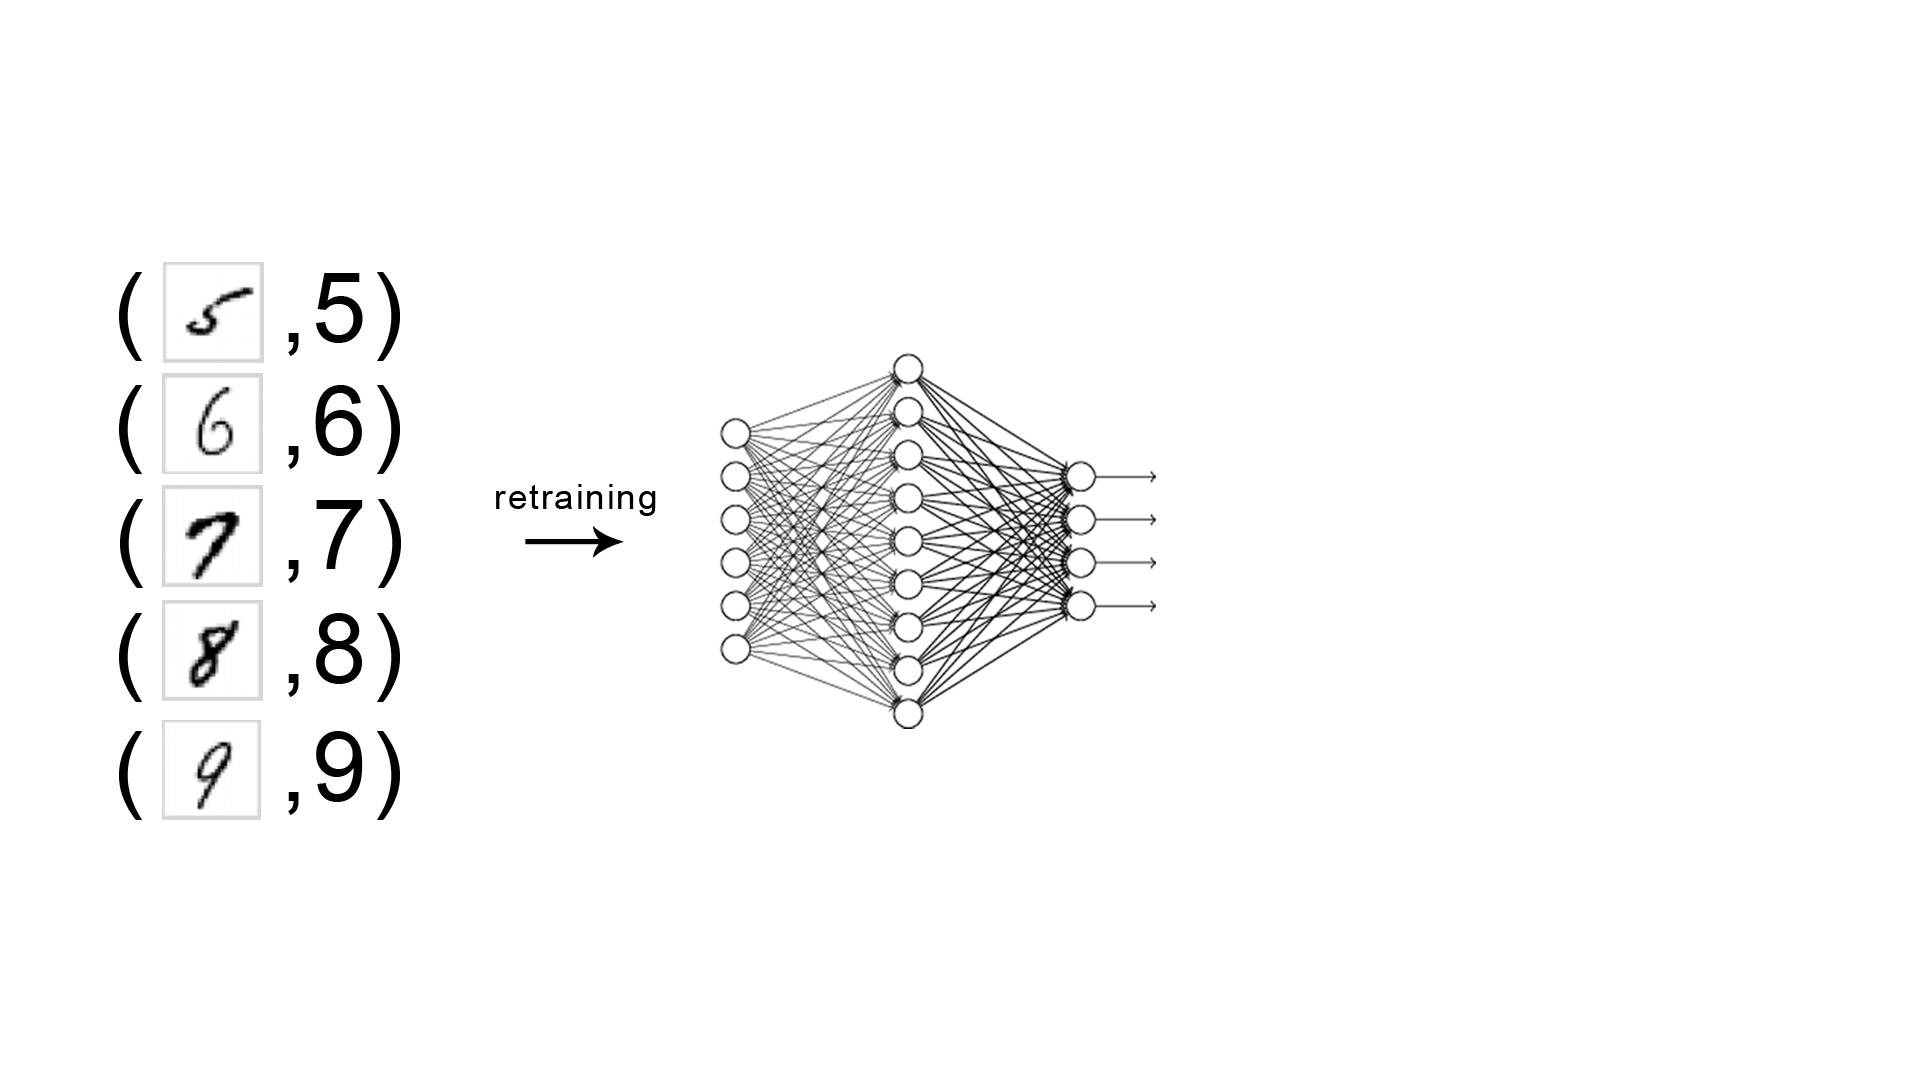
\includegraphics[width=\textwidth]{retraining_preview}
            \end{figure}
        \end{frame}
        \begin{frame}
            \frametitle{Neural Network}
            \framesubtitle{Retraining}

            \begin{figure}[H]
                \centering
                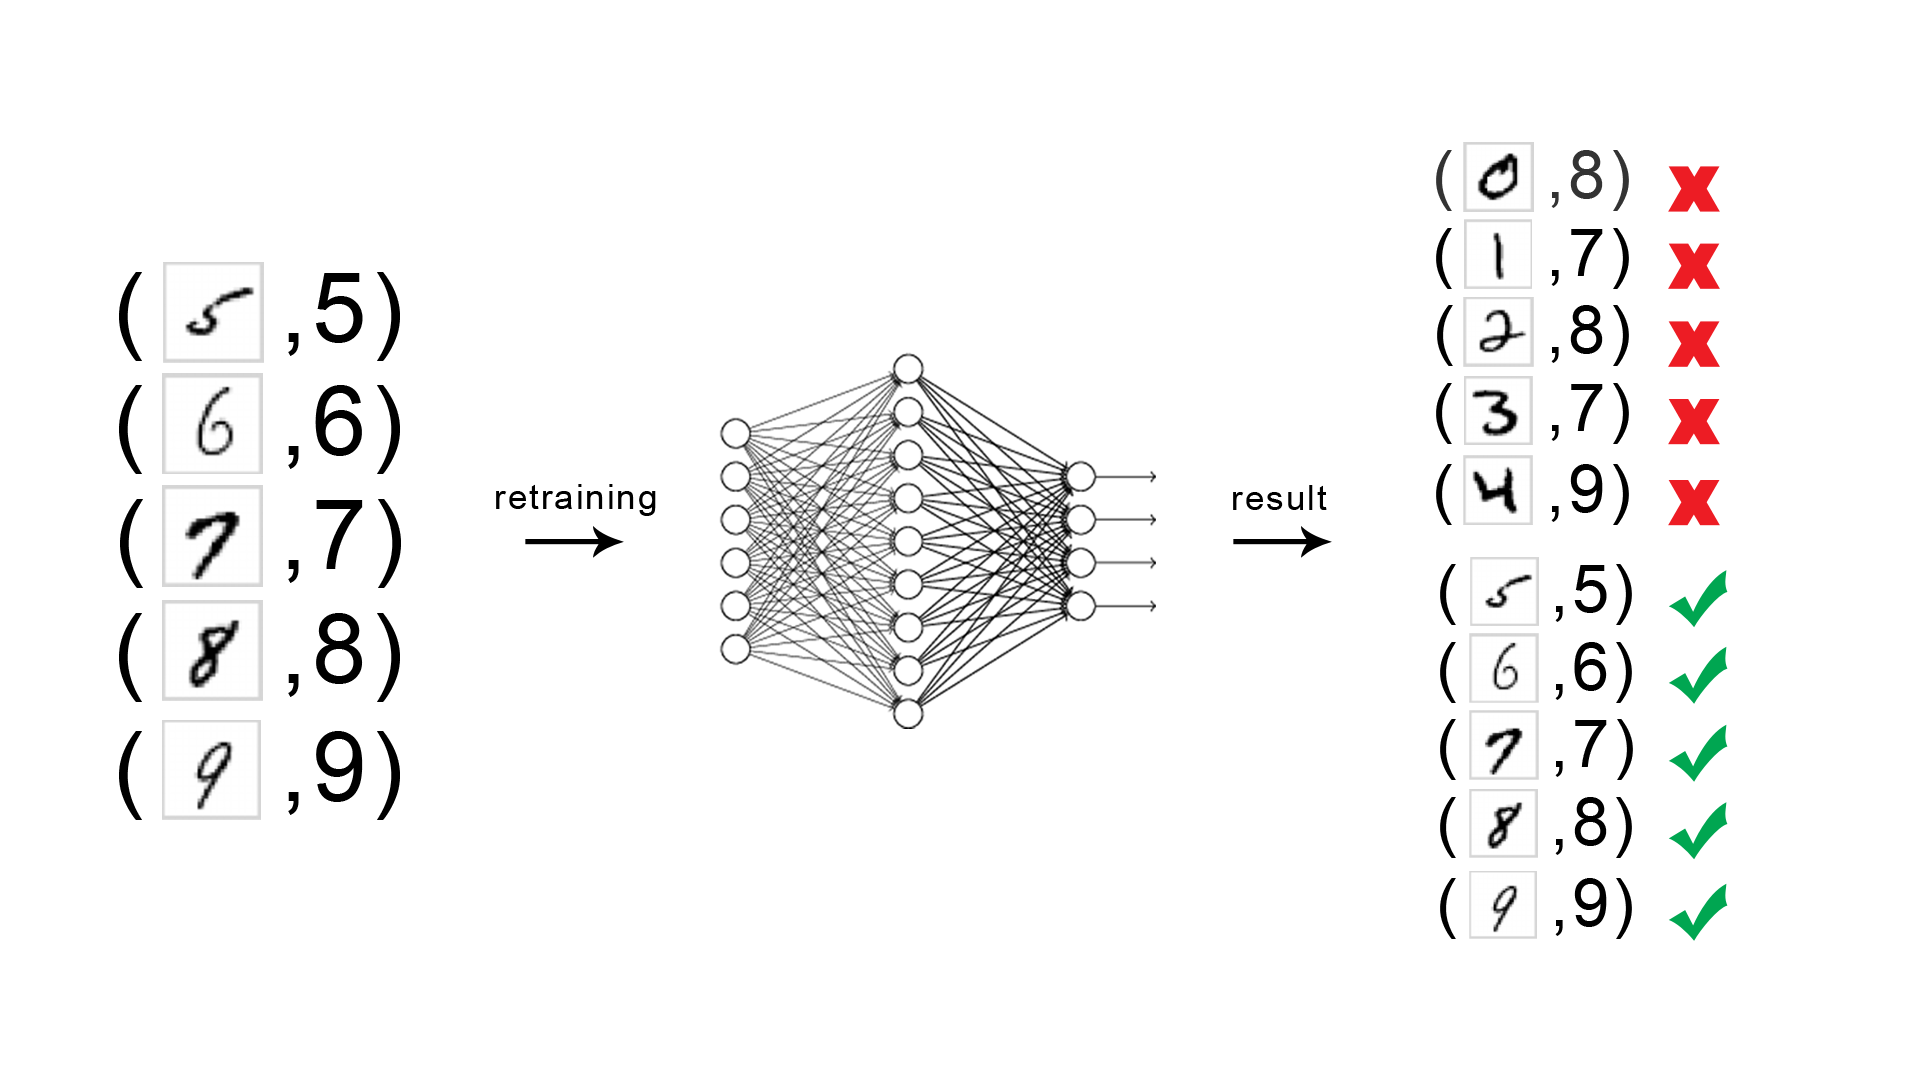
\includegraphics[width=\textwidth]{retraining_result}
            \end{figure}
        \end{frame}


        \begin{frame}
            \frametitle{Catastrophic Forgetting}
            \framesubtitle{Timeline}

            \begin{figure}[H]
                \centering
                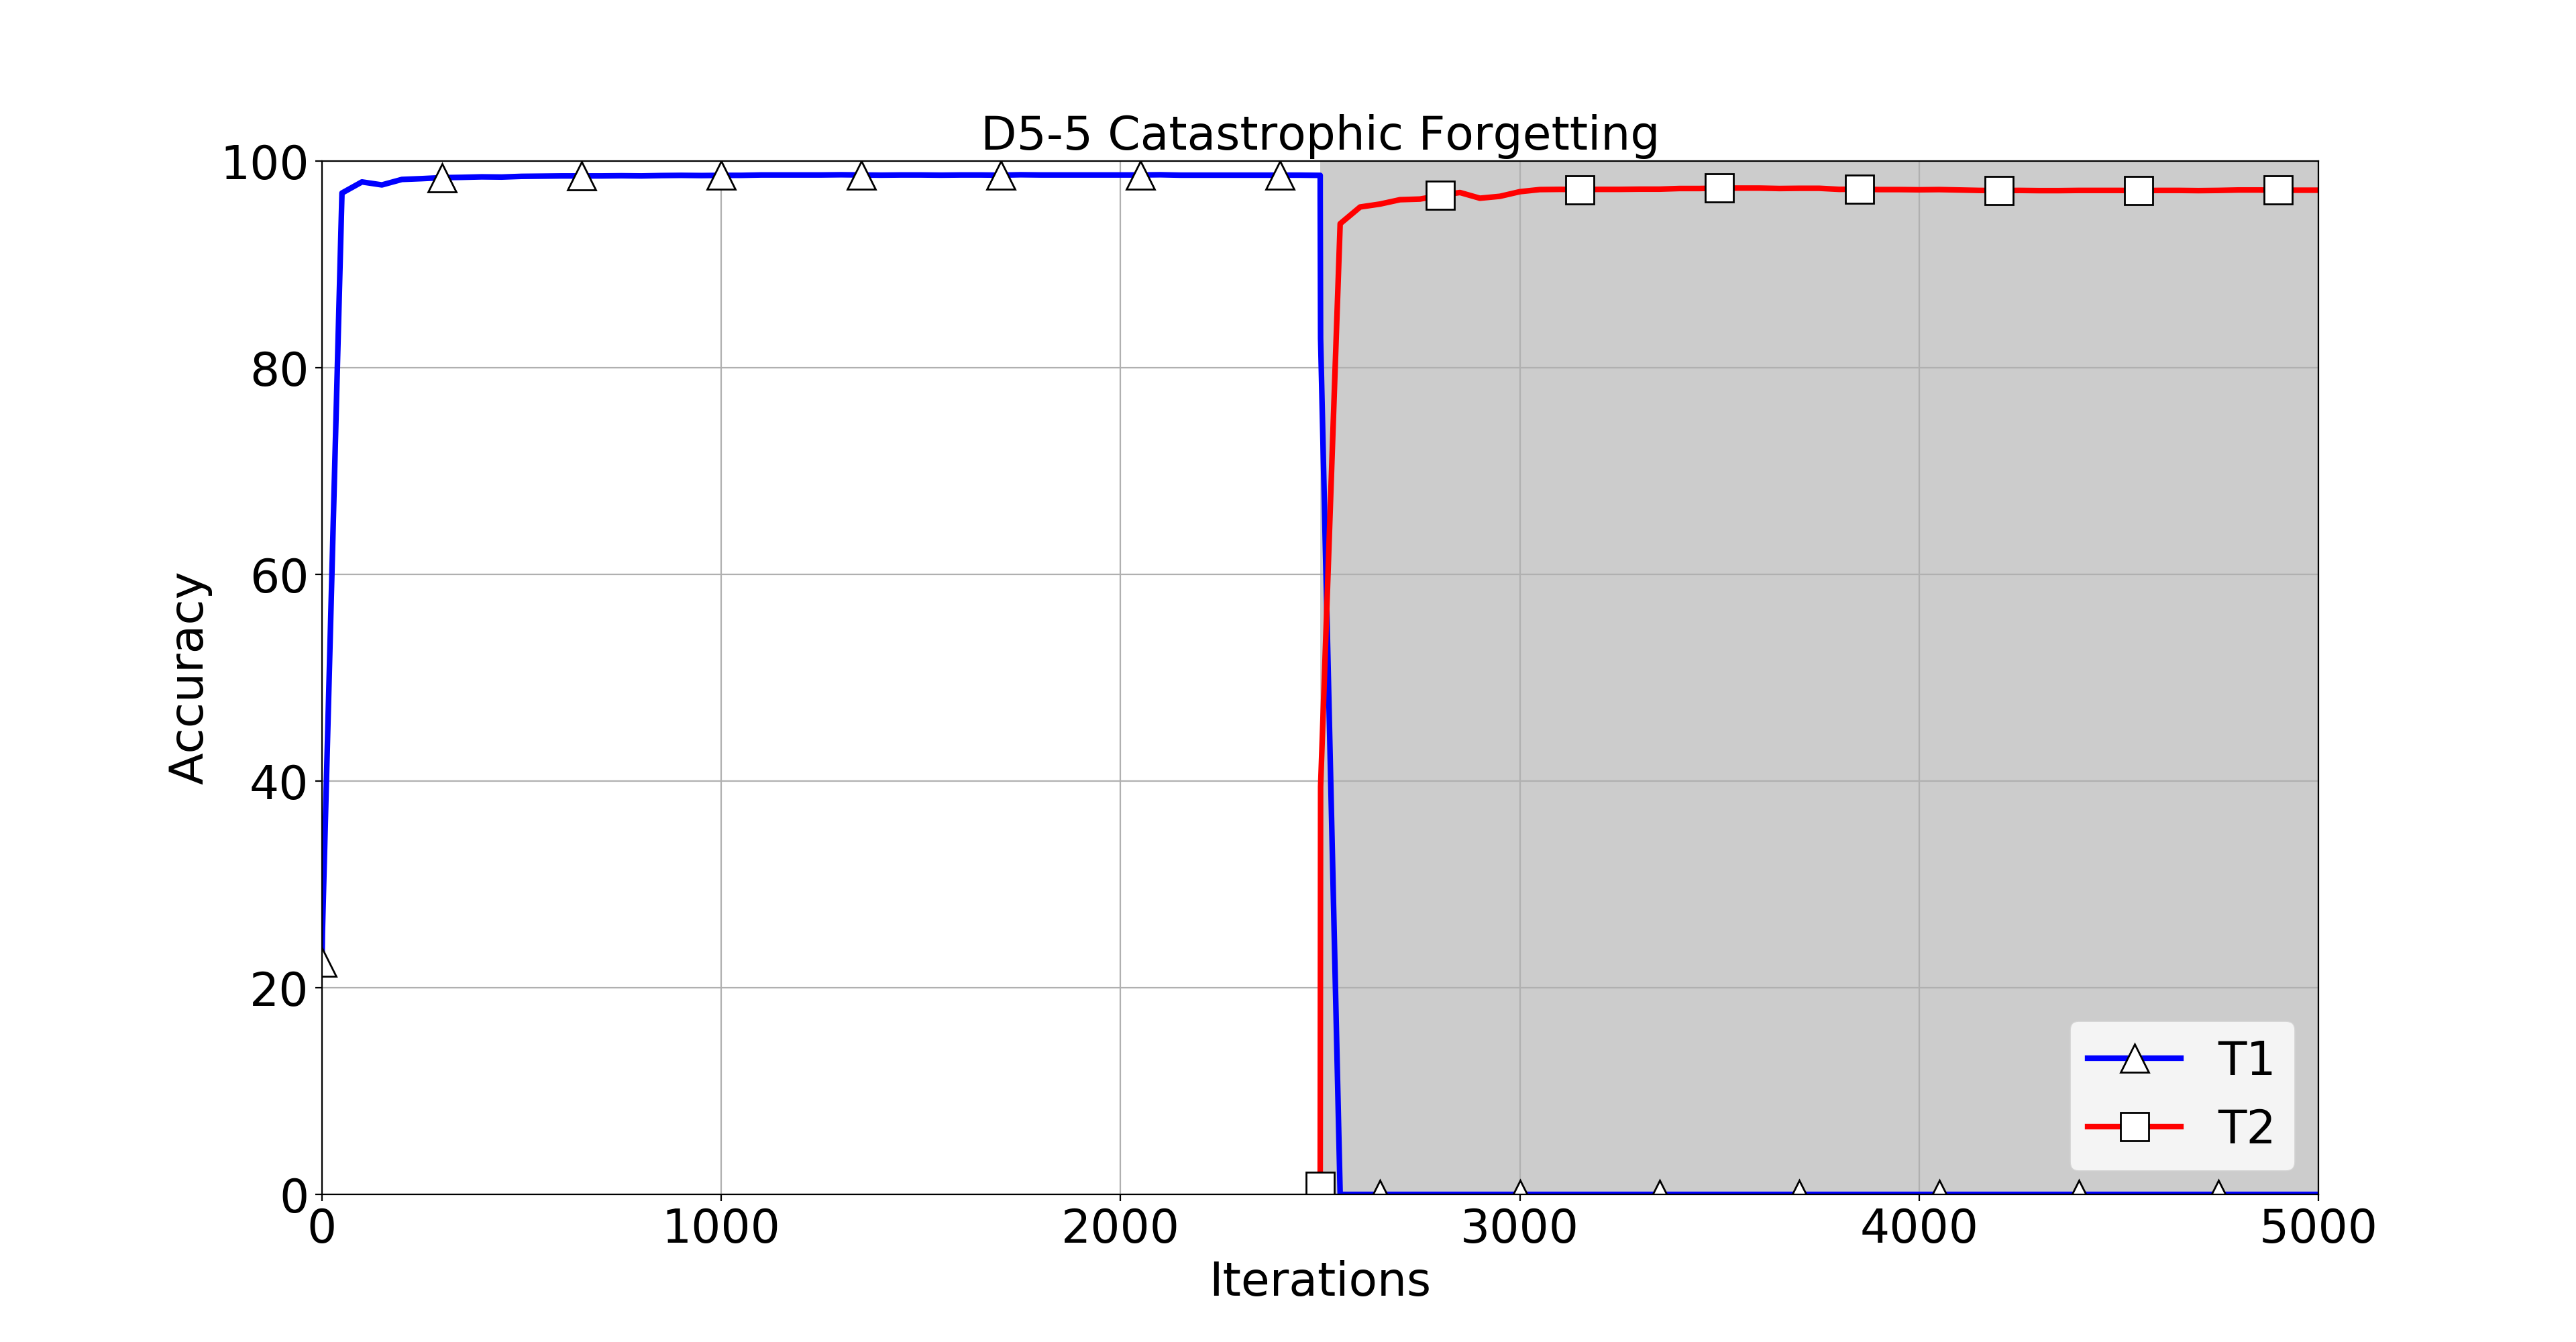
\includegraphics[width=\textwidth]{D55_catastrophic_forgetting}
                \caption{training (T1) \& retraining (T2)}
                \label{fig:CF_D55}
            \end{figure}
        \end{frame}

        \subsection{Importance of Catastrophic Forgetting}
        \begin{frame}
            \frametitle{Catastrophic Forgetting}
            \framesubtitle{Why is it important?}

            \begin{figure}[H]
                \centering
                
\includegraphics[width=\textwidth]{cf_importance}
                \label{fig:cf_importance}
            \end{figure}
        \end{frame}

        \subsection{Related Work}
        \begin{frame}
            \frametitle{Related Work}
            
            \begin{figure}[H]
                \centering
                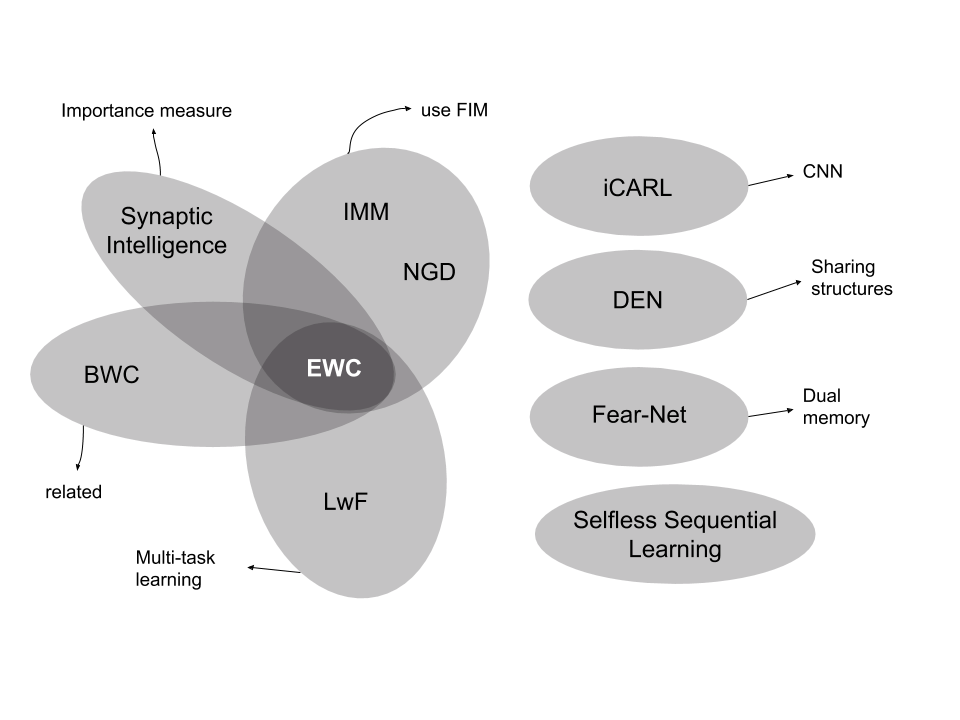
\includegraphics[width=\textwidth]{related_work}
                \label{fig:related_work}
            \end{figure}
        \end{frame}